In the coming chapter will the results of the research project be presented. First, will be diven into the architecture of web browsers. This will mostly be about the different process models and network stacks of the populair browsers. This was a prerequisite for the design and development of our algorithm that will be described in the second part of this chapter. In the last part of this chapter will be focussed on the results of the implemention and usage of the algorithm to detect real malware \todo{Better description} in a fast and reliable way.

\subsection{Web browser architectures}

Which techniques are used by browsers to make concurrently visiting multiple
URLs possible?
	- Tabs of course
		- As a process
		- As multiple threads under the browser process

How can we link an HTTP request to its source URL without the modification of the used web browser?
we need extra information, see vraag 4
network is niet genoeg blablabla

How do web browsers make HTTP requests and retrieve webpages? Which Operating System level APIs are used?
	- Safari: CFNetwork and NSURLConnection(Loader) and IPC
		1 hoofdprocess: Safari
		1 process per tab: Safari Web Content
		1 process voor networking: Safari Networking
		Network stack of OS X.
	- Internet Explorer: C API calls naar Windows libraries
		Process per tab: is configureerbaar in settings/registry, je kan ook meerdere tabs in 1 process hebben
		Network stack of Windows
	- Firefox: C++ Library calls
		Single Process (+ 1 process voor flash)
		Own network stack Necko (nss3 voor trafiek te encrypten)
		\url{https://developer.mozilla.org/en-US/Firefox/Releases/3.5/Updating_extensions#Getting_a_load_context_from_a_request}
		http://stackoverflow.com/questions/10719606/is-it-possible-to-know-the-target-domwindow-for-an-httprequest
	- Chrome: IPC 
		1 hoofdprocess: Google Chrome die networking doet
		1 process per tab. (Altijd 13 threads?)
		1 process voor Flash.
		1 process voor Audio. (4 threads)
		Own network stack (nss3 voor trafiek te encrypten)
		http://www.chromium.org/developers/design-documents/network-stack

What extra information from the client's (running) machine can be used to augment the information gained from network trac to make the tracking of malware to its source URL easier?  
	- The Thread ID or Process ID van tabs, PDF reader, Java applet, ...
	- Handle bij IE
	- File descriptors
	- Process tree
	- Voordeel van op machine network traffic te intercepten is dat we rommel van andere applicaties niet zien, maar enkel het trafiek van de browser en de gespawnde subprocessen ervan.
	- 

\subsection{Algorithm}

\begin{figure}[h]
    \centering
    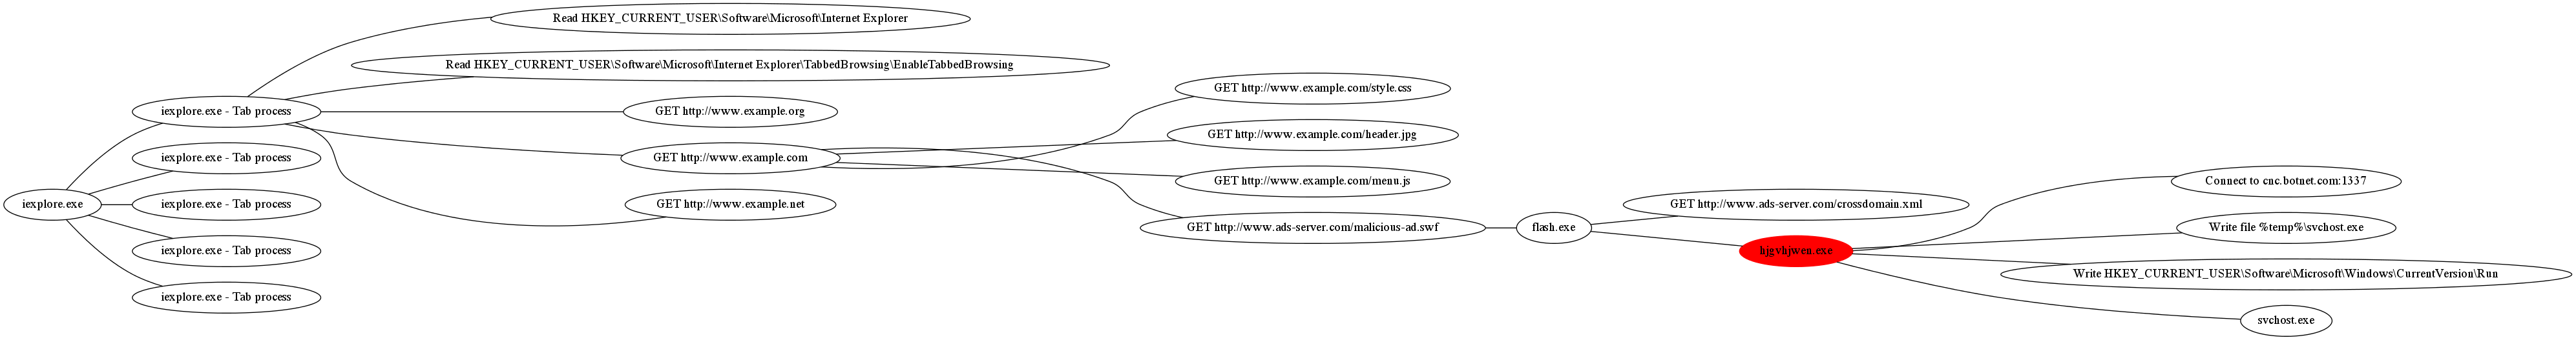
\includegraphics[width=17cm]{Images/alg_tree.png}
    \caption{An example of the graph}
    \label{fig:alg_tree}
\end{figure}

\subsubsection{Design considerations}

\subsubsection{Generic algorithm}

- Disconnected DAGs

1) Hooker schrijven voor elke browser die trafiek tussen Netwerk en Browser of in de browser zelf monitort en doorgeeft aan Cuckoo
2) DAG opstellen door de extra informatie te gebruiken in report.json
3) DAG interpreteren, nodes met enkel uitgaande edges zijn de beginnende URL
4) Kijken of er iets raar gebeurt in elk eiland
5) Reporting

\subsubsection{Platform-specific challenges}

Unix heeft geen handles zoals Windows maar meer files
	- FD's eigenlijk

\subsubsection{Alternative approaches}

- pcap / mitm
- tijd based
- aangepaste headers

\subsection{Proof of Concept}
- Waarom Cuckoo gekozen?

Speedboost tussen Cuckoo 1.2-dev en onze wijzigingen, grafiekjes maken

Problemen:

- Out of order openen en sluiten van handles 
- Paralellizatie problemen
- BSON file loggen naar de host
- COM (CrossZoneCompare, blocking Navigate met deadlock tot gevolg, )